\documentclass[10pt]{beamer}

% --- Theme Settings ---
\usetheme{Madrid}
\useoutertheme{miniframes} % Adds a sleek navigation bar at the top
\useinnertheme{circles}

% --- Custom Premium Color Palette ---
\definecolor{deepblue}{RGB}{20, 50, 110}
\definecolor{slategrey}{RGB}{80, 95, 115}
\definecolor{accentred}{RGB}{190, 40, 40}
\definecolor{softbg}{RGB}{245, 247, 250}

\usecolortheme[named=deepblue]{structure}
\setbeamercolor{palette primary}{bg=deepblue, fg=white}
\setbeamercolor{palette secondary}{bg=slategrey, fg=white}
\setbeamercolor{palette tertiary}{bg=deepblue, fg=white}
\setbeamercolor{background canvas}{bg=white}

% --- Core System Packages ---
\usepackage[utf8]{inputenc}
\usepackage[T1]{fontenc}
\usepackage{graphicx}
\usepackage{booktabs}
\usepackage{array}

% --- Graphics & Visualization ---
\usepackage{tikz}
\usetikzlibrary{shapes, arrows, positioning, shapes.geometric, calc}

% --- Code Snippet Settings ---
\usepackage{listings}
\lstset{
    basicstyle=\ttfamily\tiny,
    keywordstyle=\color{blue}\bfseries,
    commentstyle=\color{green!60!black},
    stringstyle=\color{orange},
    numbers=left,
    numberstyle=\tiny\color{gray},
    stepnumber=1,
    numbersep=5pt,
    backgroundcolor=\color{gray!5},
    showspaces=false,
    showstringspaces=false,
    showtabs=false,
    frame=single,
    rulecolor=\color{black!20},
    tabsize=2,
    breaklines=true,
    breakatwhitespace=true
}

% --- Presentation Metadata ---
\title[Seasonal Job Mobile Client]{Seasonal Job Matching Platform}
\subtitle{Mobile Client Application (\texttt{job\_seeker})}
\author[Graduation Project]{Graduation Project Defense}
\institute[Dept. of Computer Engineering]{
    Department of Computer Engineering\\
    Faculty of Engineering
}
\date[July 2026]{July 2026}

\begin{document}

% =========================================================================
% Slide 1: Title Slide
% =========================================================================
\begin{frame}[plain]
    \titlepage
\end{frame}

% =========================================================================
% Slide 2: The Mobile Seasonal Job Challenge
% =========================================================================
\begin{frame}{The Mobile Seasonal Job Challenge}
    \begin{columns}
        \begin{column}{0.5\textwidth}
            \textbf{Generic Job Portals Gaps:}
            \begin{itemize}
                \item Heavy JSON payloads draining battery.
                \item Session cache leakage on shared mobile devices.
                \item Standard store distribution delays (1--7 days for reviews).
                \item Flat rendering causing graphic frame jank.
            \end{itemize}
        \end{column}
        \begin{column}{0.5\textwidth}
            \textbf{Seasonal Job Constraints:}
            \begin{itemize}
                \item \color{accentred}Erratic Mobile Networks
                \item \color{accentred}Device Sharing Habits
                \item \color{accentred}Critical Security Patches
                \item \color{accentred}Low-End Device Hardware
            \end{itemize}
            \vspace{0.1in}
            \begin{block}{Core Objective}
                Develop a secure, optimized, and self-contained version-checking client application.
            \end{block}
        \end{column}
    \end{columns}
\end{frame}

% =========================================================================
% Slide 3: Project Scope \& Overview
% =========================================================================
\begin{frame}{Project Scope \& System Overview}
    \begin{columns}
        \begin{column}{0.4\textwidth}
            \textbf{System Scope Boundaries:}
            \begin{itemize}
                \item \textbf{In Scope:} Flutter application, secure storage, check services, updates checker.
                \item \textbf{Out of Scope:} Recruiter dashboard, Spring Boot API code, PostgreSQL management.
            \end{itemize}
        \end{column}
        \begin{column}{0.6\textwidth}
            \begin{center}
                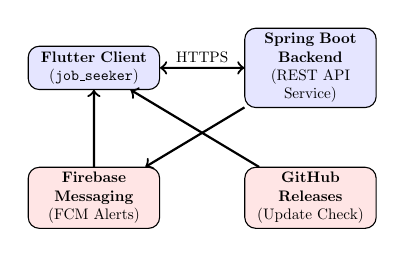
\begin{tikzpicture}[scale=0.55, every node/.style={transform shape}]
                    \tikzstyle{box} = [draw, rectangle, fill=blue!10, text width=2.8cm, minimum height=1.0cm, align=center, rounded corners]
                    \tikzstyle{cloud} = [draw, rectangle, fill=red!10, text width=2.8cm, minimum height=1.0cm, align=center, rounded corners]
                    
                    \node[box] (client) at (0, 3) {\textbf{Flutter Client}\\(\texttt{job\_seeker})};
                    \node[box] (backend) at (5, 3) {\textbf{Spring Boot Backend}\\(REST API Service)};
                    \node[cloud] (fcm) at (0, 0) {\textbf{Firebase Messaging}\\(FCM Alerts)};
                    \node[cloud] (github) at (5, 0) {\textbf{GitHub Releases}\\(Update Check)};
                    
                    \draw[<->, thick] (client) -- node[midway, above] {HTTPS} (backend);
                    \draw[->, thick] (fcm) -- (client);
                    \draw[->, thick] (github) -- (client);
                    \draw[->, thick] (backend) -- (fcm);
                \end{tikzpicture}
            \end{center}
        \end{column}
    \end{columns}
\end{frame}

% =========================================================================
% Slide 4: Internal Blueprint: Clean + MVVM
% =========================================================================
\begin{frame}{Internal Blueprint: Clean Architecture + MVVM}
    \begin{center}
        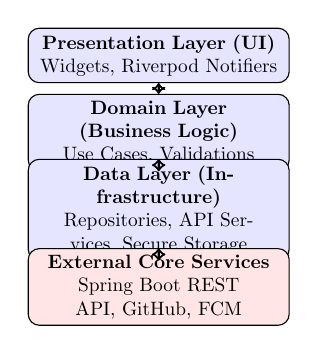
\begin{tikzpicture}[scale=0.7, every node/.style={transform shape}]
            \tikzstyle{layer} = [draw, rectangle, fill=blue!10, text width=4.5cm, minimum height=0.9cm, align=center, rounded corners]
            \tikzstyle{infra} = [draw, rectangle, fill=red!10, text width=4.5cm, minimum height=0.9cm, align=center, rounded corners]
            
            \node[layer] (pres) at (0, 3.6) {\textbf{Presentation Layer (UI)}\\Widgets, Riverpod Notifiers};
            \node[layer] (domain) at (0, 2.2) {\textbf{Domain Layer (Business Logic)}\\Use Cases, Validations};
            \node[layer] (data) at (0, 0.8) {\textbf{Data Layer (Infrastructure)}\\Repositories, API Services, Secure Storage};
            \node[infra] (external) at (0, -0.6) {\textbf{External Core Services}\\Spring Boot REST API, GitHub, FCM};
            
            \draw[<->, thick] (pres) -- (domain);
            \draw[<->, thick] (domain) -- (data);
            \draw[<->, thick] (data) -- (external);
        \end{tikzpicture}
    \end{center}
    \begin{itemize}
        \item \textbf{Decoupling:} View widgets never call the network client directly.
        \item \textbf{Riverpod State Bindings:} ViewModels expose immutable states reactively.
    \end{itemize}
\end{frame}

% =========================================================================
% Slide 5: Screen Navigation \& Branching Flow
% =========================================================================
\begin{frame}{Screen Navigation \& Branching Flow}
    \begin{center}
        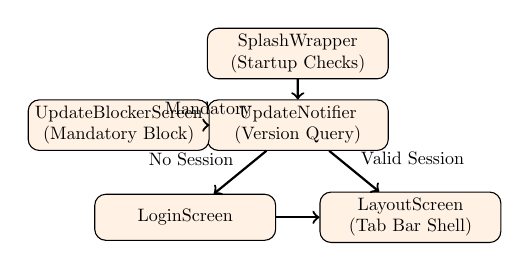
\begin{tikzpicture}[scale=0.65, every node/.style={transform shape}]
            \tikzstyle{state} = [draw, rectangle, fill=orange!10, text width=3.3cm, minimum height=0.9cm, align=center, rounded corners]
            
            \node[state] (splash) at (0, 4.2) {SplashWrapper\\(Startup Checks)};
            \node[state] (update_check) at (0, 2.8) {UpdateNotifier\\(Version Query)};
            \node[state] (blocker) at (-3.5, 2.8) {UpdateBlockerScreen\\(Mandatory Block)};
            \node[state] (login) at (-2.2, 1.0) {LoginScreen};
            \node[state] (layout) at (2.2, 1.0) {LayoutScreen\\(Tab Bar Shell)};
            
            \draw[->, thick] (splash) -- (update_check);
            \draw[->, thick] (update_check) -- node[midway, above] {Mandatory} (blocker);
            \draw[->, thick] (update_check) -- node[midway, above left] {No Session} (login);
            \draw[->, thick] (update_check) -- node[midway, above right] {Valid Session} (layout);
            \draw[->, thick] (login) -- (layout);
        \end{tikzpicture}
    \end{center}
    \begin{itemize}
        \item \textbf{Mandatory Blocker:} Prevents outdated database schema writes.
        \item \textbf{Smooth Routing:} Automatically branches to Shell navigation tabs.
    \end{itemize}
\end{frame}

% =========================================================================
% Slide 6: Session Security \& Interceptor Logic
% =========================================================================
\begin{frame}[fragile]{Session Security \& Interceptor Logic}
    \begin{lstlisting}[language=Java, caption={Dio Session Expiration Interceptor}]
dio.interceptors.add(
  InterceptorsWrapper(
    onError: (error, handler) async {
      if (error.response?.statusCode == 401 || error.response?.statusCode == 403) {
        if (AuthDialogManager().isSessionExpiredHandled) {
          handler.next(error); // Block duplicate popup alerts
          return;
        }
        AuthDialogManager().markSessionExpiredHandled();
        await storage.clearToken();
        await storage.clearUserId();
        ref.read(authProvider.notifier).logout(sessionExpired: true);
      }
      handler.next(error);
    },
  ),
);
    \end{lstlisting}
    \begin{itemize}
        \item \textbf{Keychain Persistence:} Encrypted token caching via Secure Storage.
        \item \textbf{Cache Isolation:} Logout resets all 13 providers instantly.
    \end{itemize}
\end{frame}

% =========================================================================
% Slide 7: Performance Optimizations
% =========================================================================
\begin{frame}{Performance Optimizations}
    \begin{columns}
        \begin{column}{0.5\textwidth}
            \textbf{Hybrid Scroll Pagination:}
            \begin{itemize}
                \item \textbf{Auto-Scroll:} Automatically loads next pages up to 200 items.
                \item \textbf{Manual Pause:} Pauses at 200 items, rendering a manual ``Load More'' button.
                \item \textbf{UI Safety:} Restricts rendering tree size to avoid memory overflow.
            \end{itemize}
        \end{column}
        \begin{column}{0.5\textwidth}
            \textbf{Parallel Aggregation:}
            \begin{itemize}
                \item \textbf{Concurrent Fetching:} Fetches four attributes concurrently using \texttt{Future.wait}:
                \begin{itemize}
                    \item User account data
                    \item Applied job identifiers
                    \item Favorite job status
                    \item Targeted interest chips
                \end{itemize}
                \item \textbf{Benefit:} TTI is bound to the single slowest endpoint.
            \end{itemize}
        \end{column}
    \end{columns}
\end{frame}

% =========================================================================
% Slide 8: GitHub Releases OTA Update System
% =========================================================================
\begin{frame}{GitHub Releases OTA Update System}
    \begin{columns}
        \begin{column}{0.5\textwidth}
            \textbf{Version Classifications:}
            \begin{itemize}
                \item \textbf{Mandatory Updates:} Major version shift or \texttt{[MANDATORY]} tag in name/body. Disables pop scope buttons.
                \item \textbf{Optional Updates:} Modal bottom sheet check. Dismissal triggers \color{accentred}{Snooze Logic}.
            \end{itemize}
        \end{column}
        \begin{column}{0.5\textwidth}
            \begin{center}
                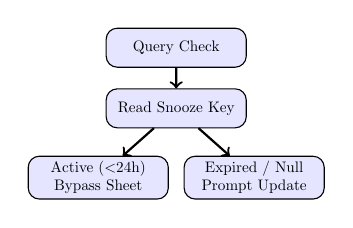
\begin{tikzpicture}[scale=0.55, every node/.style={transform shape}]
                    \tikzstyle{state} = [draw, rectangle, fill=blue!10, text width=3.0cm, minimum height=0.9cm, align=center, rounded corners]
                    \node[state] (check) at (0, 3.6) {Query Check};
                    \node[state] (snooze) at (0, 2.2) {Read Snooze Key};
                    \node[state] (active) at (-1.8, 0.6) {Active ($<$24h)\\Bypass Sheet};
                    \node[state] (expired) at (1.8, 0.6) {Expired / Null\\Prompt Update};
                    
                    \draw[->, thick] (check) -- (snooze);
                    \draw[->, thick] (snooze) -- (active);
                    \draw[->, thick] (snooze) -- (expired);
                \end{tikzpicture}
            \end{center}
        \end{column}
    \end{columns}
\end{frame}

% =========================================================================
% Slide 9: In-App Bug Reporting \& Anonymous Feedback
% =========================================================================
\begin{frame}{In-App Bug Reporting \& Anonymous Feedback}
    \begin{columns}
        \begin{column}{0.5\textwidth}
            \textbf{Anonymity Filter Logic:}
            \begin{itemize}
                \item \textbf{Send Anonymously (Checked):}
                \begin{itemize}
                    \item Omits \texttt{userEmail} from request body payload.
                \end{itemize}
                \item \textbf{Send Anonymously (Unchecked):}
                \begin{itemize}
                    \item Resolves user email from profile cache automatically.
                \end{itemize}
            \end{itemize}
        \end{column}
        \begin{column}{0.5\textwidth}
            \begin{block}{JSON Request Payload Shape}
                \texttt{\{\\
                \quad "title": "Crash on resume upload",\\
                \quad "body": "App froze during educations write",\\
                \quad \color{accentred}{"userEmail": "user@domain.com" // (Optional)}\\
                \}}
            \end{block}
            \begin{itemize}
                \item \textbf{Notifier State:} Riverpod \texttt{AsyncNotifier} manages loading spinner overlays.
            \end{itemize}
        \end{column}
    \end{columns}
\end{frame}

% =========================================================================
% Slide 10: State Engine Benchmarks \& Memory Limits
% =========================================================================
\begin{frame}{State Engine Benchmarks \& Memory Limits}
    \begin{table}[htbp]
        \centering
        \caption{Riverpod State Engine CPU Latency}
        \begin{tabular}{llc}
            \toprule
            \textbf{Data Scale} & \textbf{CPU Execution Latency} & \textbf{Safety Rating} \\
            \midrule
            100 Jobs & $\approx 0.15$ ms & Excellent \\
            1,000 Jobs & $\approx 1.25$ ms & Excellent \\
            10,000 Jobs & $\approx 8.10$ ms & Good \\
            \textbf{100,000 Jobs} & $\mathbf{\approx 14.50}$ \textbf{ms} & \textbf{Safe ($<16.6$ ms)} \\
            \bottomrule
        \end{tabular}
    \end{table}
    \begin{table}[htbp]
        \centering
        \caption{Projected Heap Memory Footprint}
        \begin{tabular}{llc}
            \toprule
            \textbf{Jobs in Heap} & \textbf{Estimated Memory Usage} & \textbf{Safety Status} \\
            \midrule
            100 Jobs & $\approx 150$ KB & Negligible \\
            1,000 Jobs & $\approx 1.5$ MB & Safe \\
            \textbf{30,000+ Jobs} & $\mathbf{\approx 45.0}$ \textbf{MB+} & \textbf{OOM Risk (Low-End)} \\
            \bottomrule
        \end{tabular}
    \end{table}
\end{frame}

% =========================================================================
% Slide 11: Testing Resilience \& Objectives Matrix
% =========================================================================
\begin{frame}{Testing Resilience \& Objectives Matrix}
    \begin{columns}
        \begin{column}{0.5\textwidth}
            \textbf{Testing Strategies:}
            \begin{itemize}
                \item \textbf{Unit Testing:} SemVer comparative algorithms, anonymous data structures.
                \item \textbf{Resilience Checks:} GitHub rate limits silent pass verification.
                \item \textbf{Secure Caching:} 24h snooze expiration clocks.
            \end{itemize}
        \end{column}
        \begin{column}{0.5\textwidth}
            \textbf{Objectives Matrix:}
            \begin{table}[htbp]
                \tiny
                \begin{tabular}{llc}
                    \toprule
                    \textbf{Objective} & \textbf{Criteria} & \textbf{Status} \\
                    \midrule
                    OBJ-SEC-1 & Token Secure Caches & PASS \\
                    OBJ-PERF-1 & TTI $\le 150\text{ms}$ (4G) & PASS \\
                    OBJ-UPD-1 & Block out updates & PASS \\
                    OBJ-CURR-1 & Currency formats & PASS \\
                    OBJ-FDBK-1 & Masked email post & PASS \\
                    \bottomrule
                \end{tabular}
            \end{table}
        \end{column}
    \end{columns}
\end{frame}

% =========================================================================
% Slide 12: Future Roadmap \& Conclusion
% =========================================================================
\begin{frame}{Future Roadmap \& Conclusion}
    \begin{itemize}
        \item \textbf{Deliverables Completed:} Decoupled Clean + MVVM Flutter application, global error session control, performance optimized pagination, and custom updates checker.
    \end{itemize}
    \vspace{0.1in}
    \textbf{Future Improvements Timeline:}
    \begin{center}
        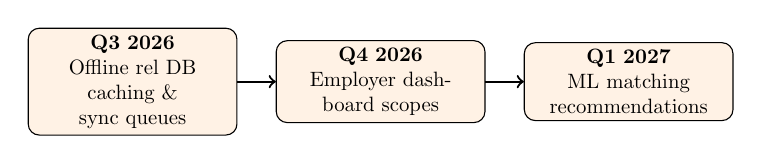
\begin{tikzpicture}[scale=0.75, every node/.style={transform shape}]
            \tikzstyle{milestone} = [draw, rectangle, fill=orange!10, text width=3.3cm, minimum height=0.8cm, align=center, rounded corners]
            
            \node[milestone] (m1) at (0, 0) {\textbf{Q3 2026}\\Offline rel DB caching \& sync queues};
            \node[milestone] (m2) at (4.2, 0) {\textbf{Q4 2026}\\Employer dashboard scopes};
            \node[milestone] (m3) at (8.4, 0) {\textbf{Q1 2027}\\ML matching recommendations};
            
            \draw[->, thick] (m1) -- (m2);
            \draw[->, thick] (m2) -- (m3);
        \end{tikzpicture}
    \end{center}
\end{frame}

% =========================================================================
% Slide 13: Acknowledgements \& Dedication
% =========================================================================
\begin{frame}{Acknowledgements \& Dedication}
    \begin{columns}
        \begin{column}{0.5\textwidth}
            \begin{block}{To My Parents \& Family}
                \small
                For their endless patience, constant encouragement, and unwavering support throughout my academic journey.
            \end{block}
        \end{column}
        \begin{column}{0.5\textwidth}
            \begin{block}{To My Supervisor \& Faculty}
                \small
                Dr. Hicham Elmongui and the Department of Computer Engineering, for their academic guidance, mentorship, and invaluable feedback.
            \end{block}
        \end{column}
    \end{columns}
    \vspace{0.4in}
    \begin{center}
        \textbf{\large Thank you. Questions \& Answers.}
    \end{center}
\end{frame}

\end{document}
